\section{Numerical Results}

Here we present a series of numerically-solved systems to illustrate the utility of the method in investigating acoustic phenomena.
We perform simulations of one- and two-particle/pulse systems to determine the principal particle-field and particle-particle interactions, followed by simulations of larger assemblages of spheres to investigate group phenomena and effects in systems without symmetry.
Unless otherwise stated, \cref{table:sim parameters} gives the simulation parameters for each of the following simulations; as our interests lie in hydrodynamic applications, we use material parameters characteristic of water to define our external fluid medium.
Similarly, we consider here the case of gas-filled \bubbles~\cite{Blomley2001}, and therefore set their density much smaller than that of the exterior medium. 
The acoustic pulses lie in the ultrasonic regime, and the chosen frequency of \SI{20}{\mega\hertz} corresponds to that of typical applications in acoustic microscopy.

\begin{table}
  \centering
  %\begin{ruledtabular}
    \begin{tabular}{lll}
      Quantity                   & Symbol   & Value                                     \\ \hline
      Sound speed                & $c_s$    & \SI{1500}{\meter \per \second}            \\
      \Bubble\ radius            & $a_k$    & \SI{1}{\micro \meter}                     \\
      Density (exterior)         & $\rho_0$ & \SI{1000}{\kilogram \per \meter \cubed}   \\
      Density (interior)         & $\rho_s$ & \SI{1}{\kilogram \per \meter \cubed}      \\
      Pulse amplitude            & $P_0$    & \SI{0.05}{\meter\squared \per \second}    \\
      Center frequency           & $f_0$    & \SIrange{0.5}{20}{\mega\hertz}            \\
      Pulse duration (st.\ dev.) & $\sigma$ & \SIrange{7}{24}{\micro\second}
    \end{tabular}
  %\end{ruledtabular}
  \caption{\label{table:sim parameters}Typical simulation parameters.}
\end{table}

\subsection{Single \bubbles}

\begin{figure}
  \centering
  \conditionalFigureInput{figures/single_particle_displacement.tex}
  \caption{\label{fig:single_displacement}Translation of a single \bubble\ interacting with an incident pulse ($f_0 = \SI{0.5}{\mega\hertz}$, $\sigma = \SI{7}{\micro\second}$). \Bubbles\ interacting with the pulse translate a finite distance along $\vb{k}$ due to the Gaussian envelope in \cref{eq:inc_field}.}
\end{figure}

\Cref{fig:single_displacement} gives the trajectory of a single \bubble\ initially at rest under the effects of an incident Gaussian pulse.
Under the linear and ideal fluid approximations and without the Gaussian envelope in \cref{eq:inc_field}, the \bubble\ merely oscillates about its origin in accordance with \cref{eq:landau result}.
In the pulsed case, however, the variation in pressure imposed by the finite value of $\vb{k}$ modifies the system dynamics to yield a net translation of each \bubble.
Note that the regime considered here produces no net transfer of momentum between the acoustic field and the \bubble---a consequence of the ideal fluid.

\begin{figure}
  \centering
  \conditionalFigureInput{figures/acoustic_trapping.tex}
  \caption{\label{fig:planar_confinement}
  (Color online) Confinement of non-interacting spheres to planes; identical counter-propagating pulses ($f_0 = \SI{20}{\mega\hertz}$, $\sigma = \SI{23.8}{\micro\second}$) initially displaced along $\vu{z}$ tend to align objects in $\nabla P = \vb{0}$ planes at $\lambda/2$ intervals.
    Here, we have sampled the field and trajectories every 30 timesteps and smoothed the resulting data with a 16-sample windowed average.
  }
\end{figure}

\Cref{fig:planar_confinement} depicts smoothed results of 128 trajectories corresponding to single \bubbles\ initially spaced along $\vu{z}$ and excited by identical counter-propagating pulses. 
By taking the width of each pulse much greater than the radius of each \bubble, the two pulses reproduce the effects of interfering standing waves. 
The confinement occurs at $\nabla P = \vb{0}$ (nodal) planes where the net force on each \bubble\ vanishes.
The half-wavelength associated with the dominant pulse frequency gives the separation between neighboring planes.

Finally, \cref{fig:dipole field} shows the relative velocity potential near a single \bubble; given a surface expansion of $\varphi$, we may compute the potential everywhere through application of \cref{eq:reduced Kirchoff-Helmholtz}.
As predicted by \cref{eq:dipole}, this field greatly resembles that of a
pointlike ``velocity dipole'' with $\vb{v}_s$ acting as a dipole moment.

The simulations described thusfar demonstrate precise acoustic control; through careful application of the incident field parameters, we may induce a (finite, given a finite pulse) translation along the principal $\vu{k}$-vector with a large degree of accuracy in the overall displacement.
In addition, the application of multiple pulses serves to confine \bubbles\ to highly localized regions in space, offering a self-consistent model of acoustic tweezing.


\begin{figure}
  \centering
  \conditionalFigureInput{figures/dipole_field.tex}
  \caption{
    \label{fig:dipole field}(Color online)
    Calculated isopotential contours near a lone \bubble.
    Red and blue colorations represent regions of positive and negative potential.
    The motion of each \bubble\ through the background medium serves primarily to produce a dipolar field of velocity potential with $\vb{v}_s$ serving as the sphere's dipole moment.
  }
\end{figure}

\subsection{Many-particle simulations}

\begin{figure}
  \centering
  \conditionalFigureInput{figures/scaling.tex}
  \caption{
    \label{fig:double scaling}(Color online)
    Scaling behavior of two \bubbles\ arranged perpendicularly to an incident pulse for various radii and initial separations.
    The (\redTriangle, \blueCircle) symbols on each axis denote data associated with that axis.
    The \redTriangle\ follow a regression of $\Delta \abs{\vb{v}}_\text{d} = \num{0.250754} d_{12}^{-3.00077}$, and the \blueCircle\ follow $\Delta\abs{\vb{v}_\text{max}}_\text{r} = \num{3.13328e-5} a_0^{2.99814}$.
    These trends strongly indicate dominant dipolar interactions between \bubbles.
  }
\end{figure}

\begin{figure}
  \centering
  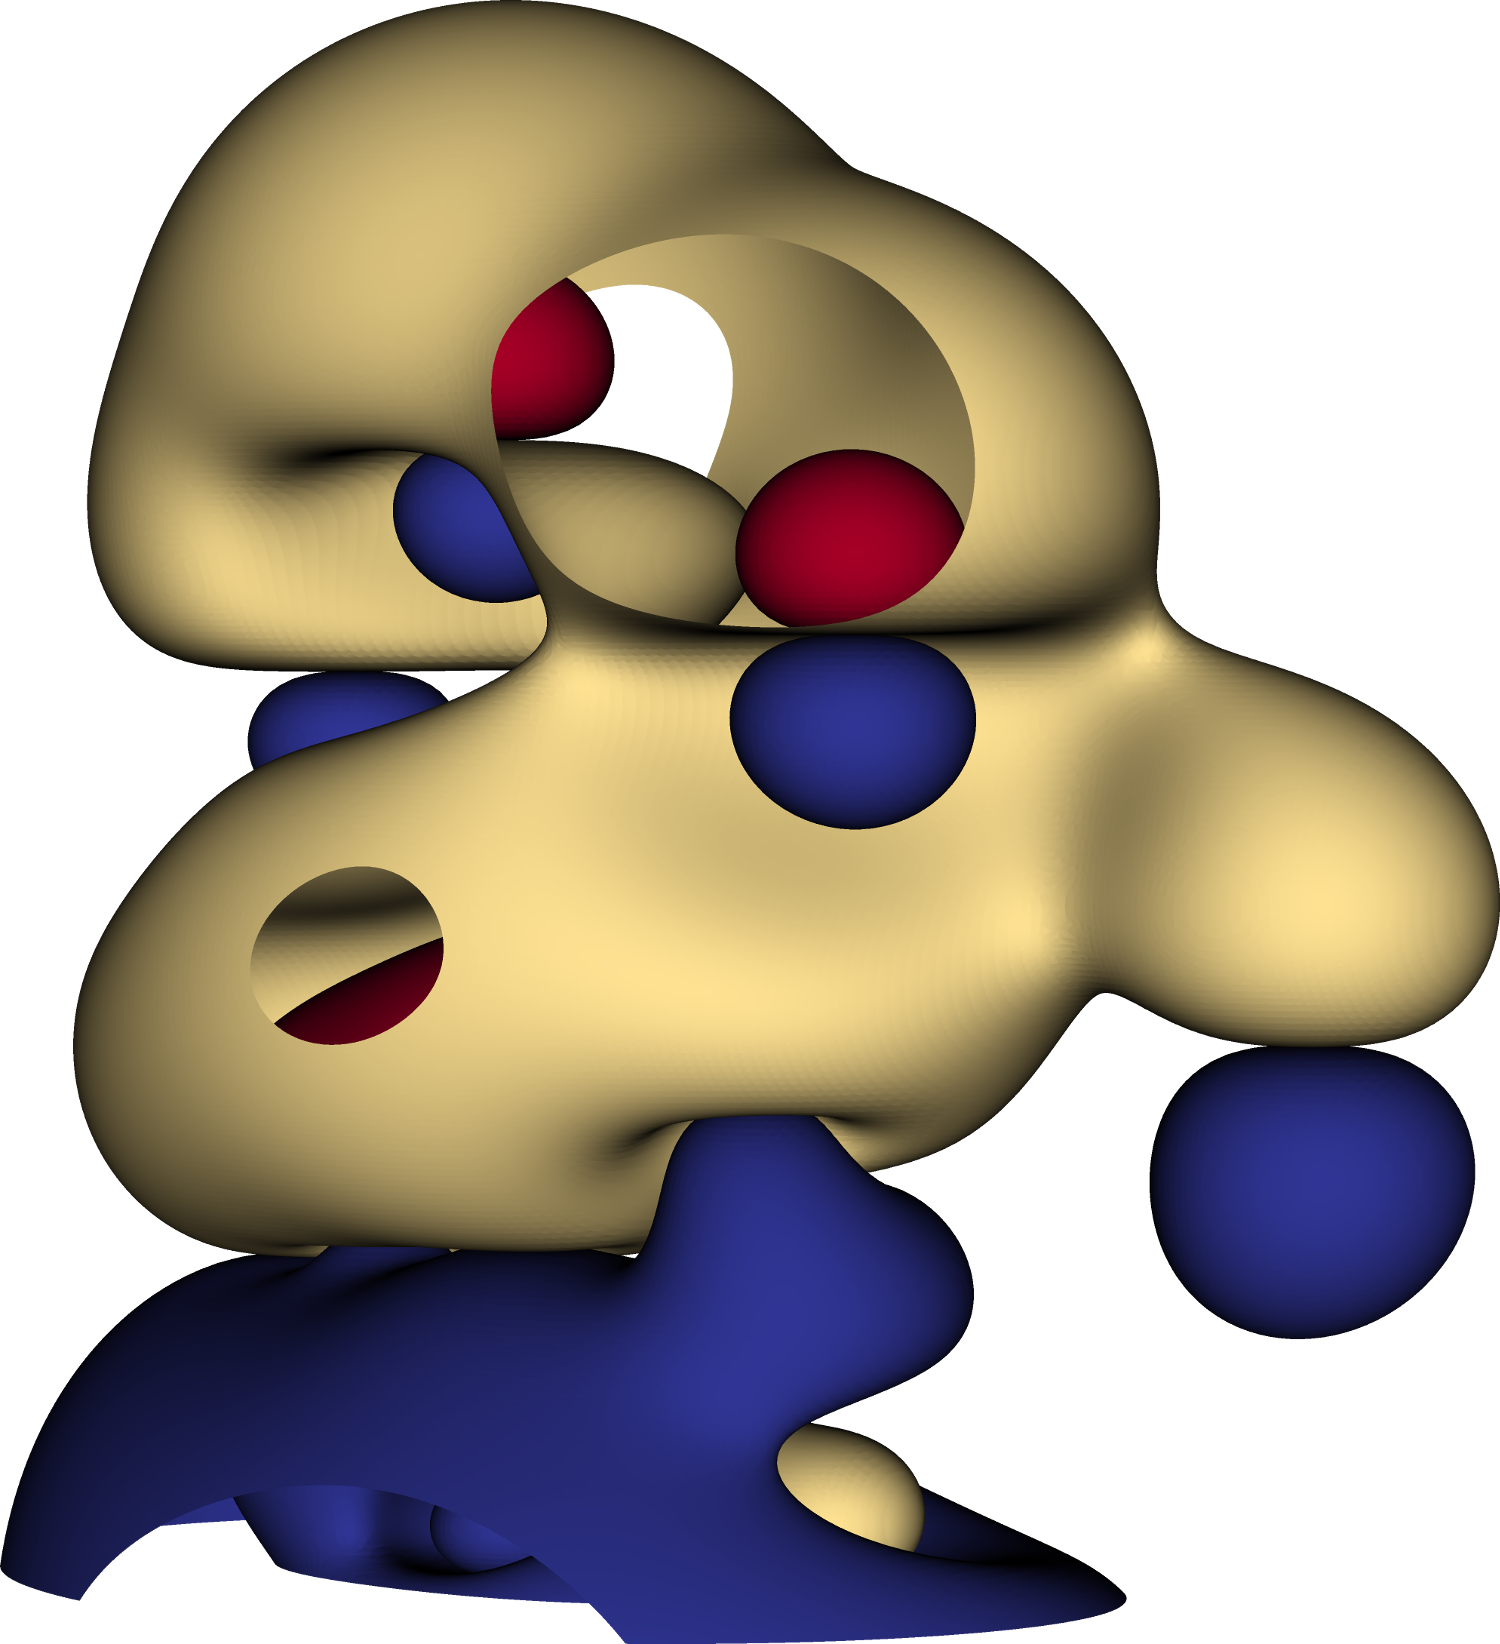
\includegraphics[width=0.5\columnwidth]{figures/3d_isosurface.png}
  \caption{
    \label{fig:isosurface}(Color online) 
    Isosurfaces of velocity potential (arb.~units) calculated by evaluating the $\hat{\mathcal{S}}$ and $\hat{\mathcal{D}}$ terms in \cref{eq:reduced Kirchoff-Helmholtz} for a $N = 16$ particle simulation.
    Red, blue, and yellow surfaces denote regions of positive, negative, and zero potential respectively, with holes appearing due to intersections with the bounding box.
    Rendered with VisIt\cite{VisIt}.
  }
\end{figure}
We now turn our attention to collections of mutually interacting \bubbles.
To quantify the effects of scattering, we first decouple scattering forces from the incident pulse by arranging two \bubbles\ perpendicularly to the pulse's $\vb{k}$-vector.
\Cref{fig:double scaling} gives results for such a simulation where we plot the relative change in velocity as compared with the single-particle simulation,
\begin{equation}
  \Delta \abs{\vb{v}_\text{max}} = \text{max}\qty(\abs{\vb{v}_\text{double}(t) - \vb{v}_\text{single}(t)}).
\end{equation}
In principle, describing quantities found from a complete simulation as a function of initial separation could obfuscate scaling data considerably; forces arising from scattering could alter the geometry of the system.
In practice, however, the perpendicular configuration used here gives scattering forces that only influence the motion along $\vb{k}$.
Consequently, $\Delta\vb{v} \propto \vb{z}$ and the \bubbles' initial separation remains a good estimator of scaling behavior. 
We see in \cref{fig:double scaling} that the radii data scale as $a_k^3$ and the
separation data exhibit strong $\abs{\vb{d}_{12}}^{-3}$ scaling, again
indicating a dominant dipolar interaction between \bubbles\ as shown by Ilinskii \etal\ in 2007~\cite{Ilinskii2007} and predicted by \cref{eq:dipole}.

Finally, we consider the dynamics of large ($N=16$) clouds of \bubbles.
For each simulation, we generate a collection of \bubbles\ initialized with zero velocity and random positions within a $\SI{10}{\micro\meter}$ ball subject to a minimum-separation constraint to prevent collisions.
\Cref{fig:isosurface} shows a snapshot of the velocity potential isosurfaces calculated in one such simulation. Even with mutual interactions, the shape of each isosurface remains consistent with the presence of a dipolar field oriented along the \bubbles' velocity.
Again, due to the localization assumption used to justify \cref{eq:green's function}, each system predominantly translates a finite distance in accordance with the results found for a single \bubble\ in \cref{fig:single_displacement}.
To quantify small changes in the geometry of a system, we compute $V_h$, the volume of the convex hull containing each \bubble, at every timestep in the simulation~\cite{SciPy}.
\Cref{fig:hull change} shows the fractional change in the hull volume,
\begin{equation}
  \Delta V_h = \frac{V_h(t) - V_h(0)}{V_h(0)},
\end{equation}
for 20 such systems after smoothing with a weighted moving average.
Curves ending above and below zero indicate larger and smaller hull volumes (system expansion and contraction).
We note from \cref{fig:hull change} a greater tendency for random clouds to expand; the effective dipole-dipole interaction between particles with $\vb{d}_{ij} \perp \vb{k}$ gives purely repulsive forces, while the interaction between particles with $\vb{d}_{ij} \parallel \vb{k}$ gives both repulsive and attractive effects depending on $\sigma$ and the relative phase of the oscillating \bubble\ velocities.

\begin{figure}
  \centering
  \conditionalFigureInput{figures/hull_percents.tex}
  \caption{\label{fig:hull change}(Color online)
    Fractional change in the volume of 20 randomly-initialized \bubble\ clouds subject to the same incident pulse, smoothed with a 128-sample moving average.
    Positive and negative values denote expansion and contraction. $\sigma = \SI{1.5}{\centi\meter}$.
  }
\end{figure}
